\chapter{Implemented Algorithms}
\label{cha:implementedAlgorithms}


%---------------------------------------------------------------------------

\section{Trend following}
\label{trend_following_impl}

The crux of the trend following method is to choose a set of entry and exit point conditions that determine our trading strategy.
Simple Moving Average (SMA) is especially useful to highlight longer-term trends in a set of data points.

SMA is formulated as the unweighted mean of the previous $N$ data points:

\begin{equation}
    SMA_{today,N} = \frac{\sum_{i=1}^{N}p_{today - i}}{N}
\end{equation}

\begin{description}
  \item [$p_{j}$] 
    value of data on day $j$
\end{description}


\textbf{Entry points:}
  \begin{itemize}
    \item Simple moving average (SMA) of last $N$ days is greater than SMA of last $M$ days
    \item Current stock price is max of last $N$ days
  \end{itemize}

As soon as at least one of the above conditions is satisfied we go long.


\textbf{Exit points:}
  \begin{itemize}
    \item Losses on a single trade are greater than 2 \% 
    \item Simple moving average (SMA) of last $N$ days is lesser than SMA of last $M$ days
  \end{itemize}

As soon as the exit condition is satisfied we go short.
 
\subsection{Pseudocode}

\begin{description}

\item[SMA(i,N)]
  calculates Simple Moving Average for stock $i$, $N$ last days are taken into account  
\item[go\_short(i)]
  sell stock $i$
\item[go\_long(i)]
  buy stock $i$
\item[get\_current\_stock\_price(i, day)]
  returns stock $i$ price for specific $day$ 
\item[get\_most\_recent\_trade\_price(i)]
  returns the price we paid for stock $i$ (we have stock $i$ in our portfolio)
\item[max(i,N)]
  returns the maximum price for stock $i$ in the last $N$ days
\item[N, M, maximal\_value\_loss]
  parameters 
\end{description}
% 


\begin{algorithmic}

\STATE $maximal\_value\_loss \gets 0.98$

\FOR{$day = 1$ to $max\_day$} 

  \FOR{$i = 1$ to $number\_of\_stocks$}

    \IF {$ get\_most\_recent\_trade\_price(i) < maximal\_value\_loss * get\_current\_stock\_price(i, day) $} 
	    \STATE $go\_short(i)$
    \ELSE
	    \IF {$SMA(i,N) < SMA(i,M)$}
		    \STATE $go\_short(i)$
	    \ENDIF
    \ENDIF

    \IF {$SMA(i,N) > SMA(i,M)$} 
	    \STATE $go\_long(i)$
    \ELSE
	    \IF {$max(i,N)) < get\_current\_stock\_price(i, day)$}
		    \STATE $go\_long(i)$
	    \ENDIF
    \ENDIF

  \ENDFOR

\ENDFOR

\end{algorithmic}

\subsection{R}

R is a programming language designed to deal with building systems based on statistical computation.
Apart from that it offers command line interpreter.
Working with vectors and matrices of data is straightforward and robust.
Its robustness and vast library of already implemented statistical functions are the main advantages of R (\cite{R}).    

\section{Genetic Algorithm}
\label{sec:genAlgoImpl}

\subsection{Adjusting GA to solve portfolio optimization problem}

As described in \ref{sec:genAlgorithms} each potential solution shoul be encoded in chromosome. 
Each chromosome represents portfolio composition (it is a vector of double values representing percentage share of each stock).

The following modified GA operations have been implemented:
\begin{description}
  \item [mutation]
      Mutation operator changes exactly one value $ \alpha_{i} $ representing percentage share of a specific stock $i$ (each time the value $i$ is chosen randomly)
      to $\alpha_{i}'$ ($\alpha_{i}' \in (0,1)$ is chosen randomly). 
      After that we have to normalize vector.
      $Mutation\_coefficient$ ($mutation\_coefficient \in (0,1)$ ) determines what part of population will be subjected to mutation operator.
  \item [selection]
      $breeding\_coefficient$ ( $breeding\_coefficient \in (0,1)$ ) determines what part of population will be subjected to crossover operator, selection is based on 
      fitness function (only the fittest part of the population will be selected)
  \item [crossover]
      After selection chromosomes eligible for reproduction, each pair of chromosomes are subjected to crossover operator. As a result new chromosomes are created (each pair
      produces two new chromosomes) and added to population. Crossover choose points $left$  and $right$ (both are chosen randomly) which cut parent's chromosomes in the following
      way: 
	  \begin{figure}[H]
	    \begin{center}
	      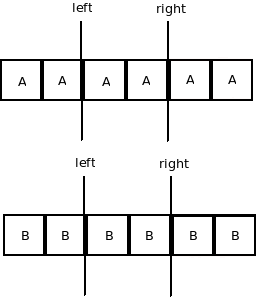
\includegraphics[scale=.4]{parents.png}
	    \end{center}
	    \caption{Example of parent's chromosomes split into 3 parts}
	  \end{figure}

	Now children are created in the following way:    
	  \begin{figure}[H]
	    \begin{center}
	      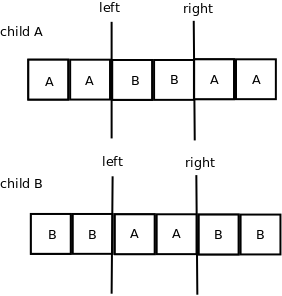
\includegraphics[scale=.4]{children.png}
	    \end{center}
	    \caption{Children's chromosomes contain mixed parent's genetic material}
	  \end{figure}

\end{description}

Apart from that, extinction mechanism has been implemented.
At the end of each GA round a part of the population that has the lowest fitness is exterminated.
$Extinction\_coefficient$ defines what part of population will be subjected to extinction.
 
\subsection{Fitness function}
\label{sec:gen_fitness_fun}

Fitness is calculated according to the following formula (for portfolio with $N$ stocks):

\begin{equation}
    \gamma_{day} =  \sum_{i=0}^{N} {  \alpha_{i} * \frac{price(i,day)}{price(i,day - 1)} }
\end{equation}

\begin{description}
  \item [$\gamma_{day}$] 
      value of the portfolio's fitness calculated for specific $day$
  \item [$\alpha_{i}$]
      percentage share of a specific stock $i$ in the whole portfolio
  \item [$price(i,day)$]
      returns the price of stock $i$ for a specific $day$
\end{description}

Clearly, the fitness function favours the portfolios which have the highest day-to-day increase in value.
Of course such method of calculating fitness has many drawbacks e.g. it completely omits the aspect of risk associated with investing in highly volatile stocks.
However, it turns out that in spite of this obvious flaw the algorithm is performing quite well.  

\subsection{Class Diagram}
\label{gen-class-diagram}

\begin{figure}[H]   
	    \begin{center}
	      \includegraphics[scale=.35]{Simple_gen_UML.png}
	    \end{center}
	    \caption{Class diagram of GA described in \ref{sec:genAlgoImpl}} 
	  \end{figure}

\begin{description}
  \item [GeneticAlgorithmImpl]
    An implementation of IGeneticAlgorithm, it is responsible for calculating the most optimal portfolio
  \item [GeneticAlgorithmUtils]
    Utility class providing methods used by genetic algorithm (like mutating, crossover etc.)
  \item [IDataSource]
    Described in \ref{dataSource}
  \item [Portfolio]
    Class representing potential solution - it stores all the information about our assets and the current value of them.

\end{description}

\section{Co-evolutionary System}
\label{sec:co-evol-sys}

\subsection{Co-evolutionary approach to portfolio optimization problem}

Contrary to \ref{sec:genAlgoImpl}, two subpopulations coexist side by side.
Each individual represent potential solution to portfolio optimization problem.
Risk oriented subpopulation tries to optimize on risk (the lower risk value the better), whereas the return oriented subpopulation tries to maximize expected return.
Usually the greater the expected return the riskier the investment so our solutions will involve some trade-offs.
However that should not startle us, as we have already predicted in \ref{sec:multi} that optimization under such circumstances is not easy.

As presented in figure~\ref{fig:co-evol}, reproduction is allowed only between members of different subpopulations.
Not every member of a particular subpopulation is allowed to reproduce - only the fittest (fitness of a particular member depends on the subpopulation it belongs to - the fittest one
 in one subpopulation would probably be considered as one of the weakest in the other one).
Thanks to this approach the offspring that is created is very diverse. 
Some part of the weakest members of both subpopulations is subjected to extinction.
Because of that we do not end up with too big population full of useless solutions.
In place of extinct members, offspring of the fittest is introduced to both subpopulations.

Apart from that, some members are subjected to mutations in order to maintain subpopulation diversity.
The migration mechanism has the same purpose - to avoid local extrema.
Risk as well as expected return are calculated according to Capital Asset Pricing Model (described in \ref{CAPM}) .


\begin{figure}[H]  
	    \begin{center}
	      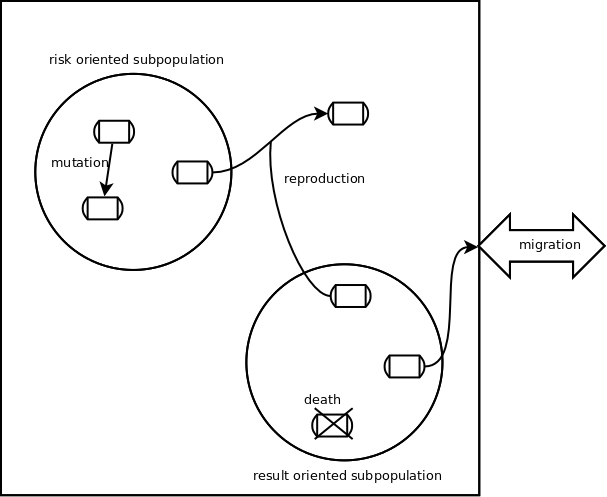
\includegraphics[scale=.35]{co-evol-2-sub.png}
	    \end{center}
	    \caption{Co-evolutionary system overview} 
	    \label{fig:co-evol}
	  \end{figure}

\subsection{Maintaining Population Diversity}

To sum up several mechanisms have been implemented to keep both subpopulations diverse:

\begin{itemize}
  \item crossover is allowed only between the fittest chromosomes from different subpopulations 
  \item mutations introducing random genetic change
  \item migration allows chromosomes to travel to different nodes  
\end{itemize}

\subsection{Class Diagram}
\label{Co-evol-class-diagram}

\begin{figure}[H]   
	    \begin{center}
	      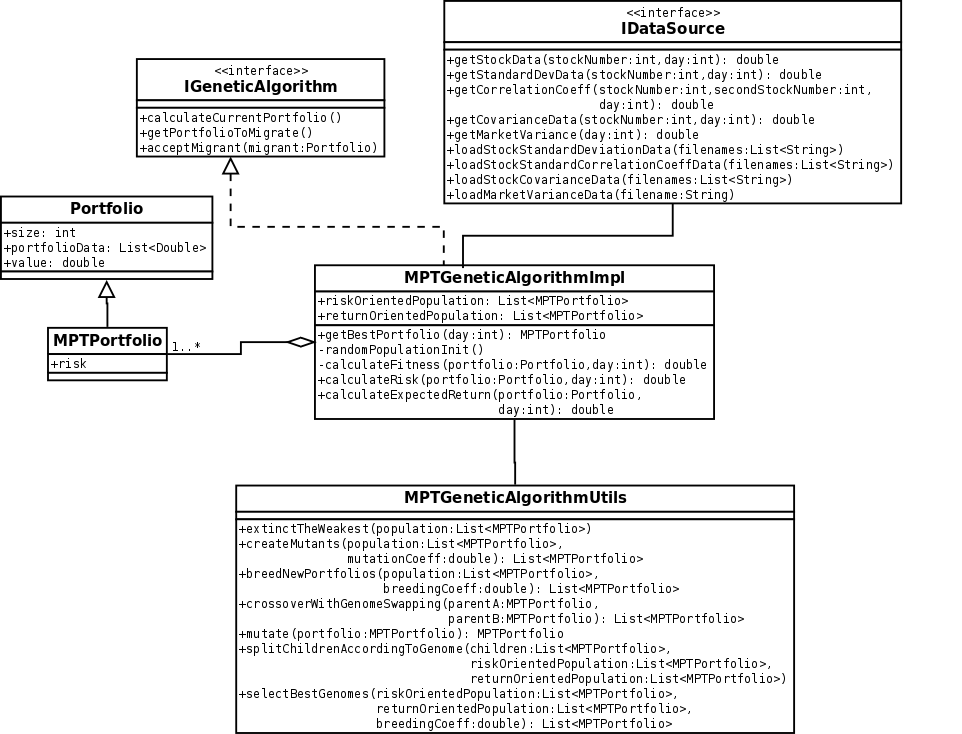
\includegraphics[scale=.35]{co-evol.png}
	    \end{center}
	    \caption{Class diagram of GA described in \ref{sec:genAlgoImpl}} 
	  \end{figure}


\section{Co-Evolutionary Multi-agent System - CoEMAS}

Co-evolutionary Multi-agent System (CoEMAS) is the most sophisticated system that has been implemented.
As described in \ref{sec:multi} and \ref{sec:co-evol} such systems need environment as well as a set of autonomous agents interacting with each other.
Potential solution to portfolio optimization problem is stored inside each agent.


\begin{figure}[H]   
	    \begin{center}
	      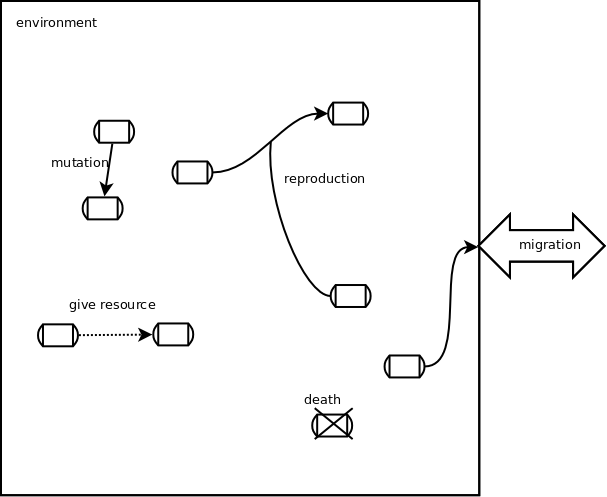
\includegraphics[scale=.38]{agent.png}
	    \end{center}
	    \caption{Overview of CoEMAS} 
	  \end{figure}

Contrary to \ref{sec:co-evol-sys} there are no subpopulations.
Instead of them we introduced individuals of two different species.
Each species focuses on different task:

\begin{itemize}
  \item species number 1 - tries to achieve the lowest risk possible
  \item species number 2 - tries to achieve the highest expected return possible
\end{itemize}

Risk as well as expected return is calculated due to Capital Asset Pricing Model (defined in \ref{CAPM}).

Implemented actions that each agent can perform include (\ref{sec:CoEMAS}):

\begin{description}
  \item [death]
      if amount of resource that agent posses is lower than threshold value the agent dies
  \item [migration]
      agent is allowed to migrate but the probability of this action is low
  \item [reproduction]
      agents from different species are allowed to reproduce provided that they both exceed the minimum amount of resource allowing to reproduce
  \item [give/get]
      agent can get resource from other, dominated agent
  \item [recombination]
      agents produce offspring by the means of recombination
  \item [mutation]
      mutation introduces random change to potential solution, normalization of solution vector is then required 
  \item [seek]
      agents appropriate  to reproduction as well as get operation can be found thanks to this action
\end{description}

Interactions between agents are implemented in the following way:
\begin{itemize}
  \item co-evolution is implemented as a sequence of \emph{turns}
  \item in each \emph{turn} every agent perform its action (action to perform at any particular turn is chosen with some well defined probability, e.g. there is a 10\% chance that agent will try to find
	a partner to reproduce, 60\% chance that the agent will try to get some resource from dominated agent)
  \item when every agent performed some action the \emph{turn} ends and entire population of agents is checked whether some of them should die (not enough resource left after other agents got resource
	from it)
\end{itemize}


Each agent performs one of the above actions with some probability.



\subsection{Class Diagram}
\label{CoEMAS-class-diagram}

\begin{figure}[H]   
	    \begin{center}
	      \includegraphics[scale=.3]{CoEMAS-UML.png}
	    \end{center}
	    \caption{Class diagram of CoEMAS} 
	  \end{figure}

\begin{description}
  \item [Environment]
      aggregates all agents, responsible for population init at the start of algorithm and extinction of agents which resource level are too low, etc.
  \item [AgentUtils]
      utility class providing functions to Agent class
  \item [IAgent]
      interface specifying all methods that agent in CoEMAS should be capable of doing
  \item [Agent]
      implementation of agent that is autonomous and interact with other agents
  \item [IDataSource]
      provides easy access to historical data and computed statistical functions
 
\end{description}


%---------------------------------------------------------------------------

\section{Implementation Details}
\label{sec:implDetails}


\subsection{Multi-agent running platform architecture}
\label{multi-agent}

%\clearpage
\begin{figure}[H]
  \begin{center}
    \includegraphics[scale=.4]{agent_framework.png}
  \end{center}
  \caption{Deployment diagram of two Computing Nodes and Aggregation Node (in real situations more Computing Nodes are present)}
\end{figure}

Data Source as well as Computing Algorithm are created and injected to Computing Node(CN) by Spring. 
CNs send results of computations to Aggregating Node by JMS. 
Apart from that, JMS is used to provide migration capability to each CN.


\subsection{Precomputation of statistical functions}
\label{precompute}
Precomputation of statistical functions (like covariance, standard deviation etc.) from historical data is done by R scripts. 
Results are stored in files, later used as an input to other algorithms.
In order to provide easy and centralised access to historical data and precomputed statistical functions Data Source component has been introduced. 

\subsection{Data Source component}
\label{dataSource}

Data Source component aggregates all stocks historical data as well as all precomputed statistical functions results from \ref{precompute}.   
Its interface enables access to all data it contains. Data Source is injected as a bean to other components by Spring.
They use it mainly as a source of data required by various algorithms.

\subsection{Computing Algorithm component}

Computing Algorithm component is responsible for carrying out all computations.
In order to function properly Data Source component as well as all configuration variables (like mutation coefficient etc.) has to be injected by Spring.
Apart from trend following algorithm, all the remaining approaches (CoEMAS (\ref{CoEMAS-class-diagram}), co-evolutionary (\ref{Co-evol-class-diagram}),
 genetic algorithm (\ref{gen-class-diagram})) can be injected to Computing Algorithm component so they can be run
 in a multi-agent system as a working horse of a Computing Node.


\subsection{Aggregating Node}

The sole purpose of Aggregating Node(AG) is to gather results from Computing Nodes(CN), choose the best non-dominated solution and write the results to file. 
Based on this file all charts are created and comparison of different algorithms is possible.
Communication between CNs and AG is provided by a single JMS queue (all CNs send results to one specific queue, AG consumes its content).


\subsection{Technologies used}

\begin{description}
  \item [R]
      Trend following algorithm has been implemented as an R script, historical data preprocessing.
  \item [Apache ActiveMQ]
      JMS implementation, provides communication between Computing Nodes and Aggregating Agent (\ref{multi-agent})
  \item [Java]
      Almost all algorithms are implemented in Java, Computing Nodes as well as Aggregating Node are in fact jar files 
  \item [Spring Framework]
      Inversion of Control container (configuration of application components and lifecycle management of Java objects), Messaging (simplifies the use of the JMS API) modules used.
  \item [Apache Maven]
      Used primarly for build automation.
  \item [JUnit]
      JUnit tests cover the most crucial functions of implemented algorithms.
  \item [git]
      Source Code Management tool.
  \item [bash scripts]
      Used for conveniently setting up and running test 
\end{description}

 